\section{面向延迟的基于参数非平稳策略优化}


\subsection{终身基于参数策略优化}
\label{sec:lifelong_param_po}

本节中，我们基于参数 \gls{po}，考虑 $\mathcal{V}_{\mathcal{P}} = \{\nu_{\vectorialform{\rho}} : \vectorialform{\rho} \in \mathcal{P} \subseteq \realnumbers^{n_\rho}\}$ 中的超策略和 $\Pi_{\Theta} = \{\pi_{\vectorialform{\theta}} : \vectorialform{\theta} \in \Theta \subseteq \realnumbers^{n_\theta}\}$ 中的策略。
为了优化 \Cref{eq:beta_steps_ahead_return} 中的 $\beta$ 步前视期望回报，策略必须是非平稳的。
这可以通过两种方式利用参数 \gls{po} 框架实现。
第一种方式，状态 $s$ 增广当前时间 $t$，得到策略 $a_t\sim\pi_{\boldsymbol\theta}(\cdot\vert(s,t))$。
这一表述清晰展示了动作对时间的依赖。
第二种方式，对时间的依赖转移到超策略层面，因此策略的参数依赖于时间 $\boldsymbol\theta_t \sim \nu_{\boldsymbol\rho}(\cdot\vert t)$。
这可以说提供了对智能体如何适应非平稳性的更好理解。
两种框架的图形表示见 \Cref{fig:graph_models}。
我们将此设定称为 \emph{终身基于参数 PO}。


\begin{figure}[t]
    \centering
    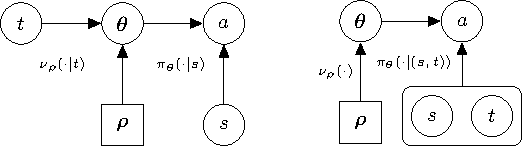
\includegraphics[labellifelong=graphparamactionbasedns]{img/thesis_plots_chapter_lifelong.pdf}
    \caption{表示将参数 \gls{po} 应用于环境非平稳性的两种框架的图形模型。左图：在策略参数层面处理非平稳性；右图：在动作层面处理非平稳性。}
    \label{fig:graph_models}
\end{figure}

$\beta$ 步前视期望回报可以针对参数 \gls{po} 重新表述为：
\begin{align}\label{eq:opt}
    \boldsymbol\rho^\star_{T,\beta} \in \argmax_{\boldsymbol\rho \in \mathcal{P}} \expectedreturn[T,\beta][](\boldsymbol\rho) = \sum_{t=T+1}^{T+\beta} \widehat{\gamma}^t \expectedvalue_t^{\boldsymbol\rho}[r_t],
\end{align}
其中 $\mathbb{E}_t^{\boldsymbol\rho}\coloneq \expectedvalue_{\boldsymbol\theta \sim \nu_{\boldsymbol\rho}(\cdot\vert t)}[\mathbb{E}_t^{\pi_{\boldsymbol\theta}}[\cdot]]$。


\subsection{通过多重重要性采样的终身基于参数 PO}
\label{subsec:mis_lifelong}

现在我们提出一种优化 $\beta$ 步前视期望回报的方法。
在 \Cref{subsec:beta_step_estim} 中，我们推导该量的估计量。
在 \Cref{subsec:bias_analysis} 中，我们分析估计量的偏差，在 \Cref{subsec:variance_analysis} 中分析其方差。
最后，在 \Cref{subsec:surrogate_objective} 中，我们提出一个替代目标，考虑估计的不确定性，以优化 $\expectedreturn[T,\beta][](\boldsymbol\rho)$ 的下界。

\subsubsection{$\beta$ 步前视期望回报估计量}
\label{subsec:beta_step_estim}

显然，这里的挑战在于估计一个依赖于未来未知动态的量，而我们只能访问过去（动态可能不同）的样本。
然而，假设非平稳性是平滑的（我们在此做出这一假设），使得利用过去动态预测未来动态变得合理。
更形式化地，令 $\mathcal{H}_{T,\alpha} = (\boldsymbol\theta_t,r_t)_{t \in [\![T-\alpha+1,T]\!]}$ 为与环境的终身交互中最后 $\alpha$ 个样本。
利用这些样本和 \gls{mis}，可以构建对 $s \in [\![T+1,T+\beta]\!]$ 的 $s$ 步前视期望奖励 $\mathbb{E}_s^{\boldsymbol\rho}[r_s]$ 的（有偏）估计量：
\begin{align*}
    \widehat{r}_{s} = \sum_{t=T-\alpha+1}^{T} \omega^{T-t} \frac{\nu_{\boldsymbol\rho}(\boldsymbol\theta_t\vert s)}{ \sum_{k=T-\alpha+1}^T \omega^{T-k} \nu_{\boldsymbol\rho}(\boldsymbol\theta_t\vert k)} r_{t},
\end{align*}
其中 $\omega \in [0,1]$ 是指数折扣参数。
注意，此处重要性采样权重 $\textstyle\frac{\nu_{\boldsymbol\rho}(\boldsymbol\theta_t\vert s)}{ \sum_{k=T-\alpha+1}^T \omega^{T-k} \nu_{\boldsymbol\rho}(\boldsymbol\theta_k\vert k)}$ 解释了未来目标超策略 $\nu_{\boldsymbol\rho}(\cdot\vert s)$ 与过去行为超策略 $\nu_{\boldsymbol\rho}(\cdot\vert k)$ 之间的差异。
由于 $\omega$ 折扣，\gls{mis} 估计量并未精确使用 BH 建议的系数（见~\Cref{subsec:importance_sampling}）。
相反，它通过给近期样本更高权重来体现我们对环境平滑变化的认识。BH 则会对每个过去样本赋予相同权重。
在非平稳环境中，对较旧样本进行指数折扣并非新方法 \cite{jagerman2019people}。

现在可以利用估计量 $\widehat{r}_{s}$ 来估计 $\beta$ 步前视期望回报，
\begin{align*}
    \widehat{J}_{T,\alpha,\beta}({\boldsymbol\rho}) &= \sum_{s=T+1}^{T+\beta} \widehat{\gamma}^{s} \widehat{r}_{s} \\
    & = \sum_{t=T-\alpha+1}^{T} \omega^{T-t} \frac{\sum_{s=T+1}^{T+\beta} \widehat{\gamma}^s \nu_{\boldsymbol\rho}(\boldsymbol\theta_t\vert s)}{\sum_{k=T-\alpha+1}^T \omega^{T-k} \nu_{\boldsymbol\rho}(\boldsymbol\theta_t\vert k)} r_{t}.
\end{align*}
该量可以直接最大化；然而，这会受到 \gls{is} 估计量的一个常见缺点的影响，我们将在下文解释。
要增加 $\widehat{J}_{T,\alpha,\beta}({\boldsymbol\rho})$，可以增加未来选择好策略的概率 $\nu_{\boldsymbol\rho}(\boldsymbol\theta_t\vert s)$（$\widehat{J}_{T,\alpha,\beta}({\boldsymbol\rho})$ 的分子），或者降低过去选择同样好策略的概率 $\nu_{\boldsymbol\rho}(\boldsymbol\theta_t\vert k)$（$\widehat{J}_{T,\alpha,\beta}({\boldsymbol\rho})$ 的分母）。
虽然第一个效果是期望的，第二个显然不是，并且相当于灾难性遗忘。
然而，可以通过简单调整来防止这种现象。
通过将最后 $\alpha$ 个奖励添加到目标函数中，智能体将避免降低过去好策略的概率。
这个添加的量，我们称为 \emph{$\alpha$ 步后视期望回报}，表示为：
\begin{align*}
    \widecheck{J}_{T,\alpha}({\boldsymbol\rho}) = \frac{1}{C_\omega(\alpha)} \sum_{t=T-\alpha+1}^{T} \omega^{T-t}  \widecheck{\gamma}^t r_{t},
\end{align*}
其中 $\widecheck{\gamma}^t = \widecheck{\gamma}^{t-T+\alpha-1}$，并且我们定义了对于 $\xi \ge 1$ 和 $\tau\in[0,1]$
\begin{align}
\label{eq:def_function_C}
C_\tau(\xi)=\left\{
\begin{array}{cc}
    \frac{1-\tau^\xi}{1-\tau} & \text{ if } \tau<1 \\
    \xi & \text{ otherwise.}
\end{array}\right.
\end{align}
新目标因此变为，
\begin{align}
\label{eq:non_yet_objective}
    \overline{J}_{T,\alpha,\beta}(\boldsymbol\rho) = \widehat{J}_{T,\alpha,\beta}({\boldsymbol\rho})  +  \widecheck{J}_{T,\alpha}({\boldsymbol\rho}).
\end{align}


\subsubsection{偏差分析}
\label{subsec:bias_analysis}

由于非平稳性，估计量 $\widehat{J}_{T,\alpha,\beta}(\boldsymbol\rho)$ 很可能有偏。
然而，我们设计它适用于平滑演化的动态。
下文我们形式化 "平滑" 的含义，并分析这些条件下估计量的偏差。

\begin{ass}[平滑非平稳环境]
\label{ass:sce}
对于任意 $t,t' \in \naturalnumbers$，以及任意策略 $\pi$，存在 Lipschitz 常数 $0 \le L_{\markovdecisionprocess} < \infty$ 使得：
\begin{align*}
    \left\vert  \left(\mathbb{E}_{t}^{\pi}-\mathbb{E}_{t'}^{\pi} \right)\left[ r \right] \right\vert  \le L_{\mathcal{M}} \lvert t - t'\rvert.
\end{align*}
\end{ass}
\begin{ass}[平滑非平稳超策略]
\label{ass:sch}
对于任意 $t,t' \in \naturalnumbers$，以及任意时间相关超策略 $\boldsymbol\rho \in \mathcal{P}$，存在 Lipschitz 常数 $0 \le L_{\nu} < \infty$ 使得：
\begin{align*}
    \left\Vert  \nu_{\boldsymbol\rho}(\cdot\vert t) - \nu_{\boldsymbol\rho}(\cdot\vert t') \right\Vert _1 \le L_{\nu} \lvert t - t'\rvert.
\end{align*}
\end{ass}

\Cref{ass:sce} 确保在两种不同时间执行相同策略所收集的期望奖励的差异受时间差的比例约束。
类似地，\Cref{ass:sch} 确保两种不同时间超策略的概率分布在总变差距离上受时间差的比例约束。
关于平滑非平稳动态的假设以简化最坏情况分析在文献中并不新鲜 \cite{lecarpentier2019non}。
利用这些假设，可以推导出偏差的以下界。
为简洁起见，我们用 $\mathbb{E}_{T,\alpha}^{\boldsymbol\rho}$ 表示由时间 $T-\alpha+1$ 到 $T$ 的超策略诱导的联合概率分布下的期望，即，
\begin{align}
\label{eq:joint_hyper_pol}
    \prod_{t=T-\alpha+1}^{T} \nu_{\boldsymbol\rho}(\cdot\vert t).
\end{align}


\begin{lemma}
\label{lem:bias_bound}
在 \Cref{ass:sce} 和 \Cref{ass:sch} 以及 $\omega<1$ 条件下，估计量 $\widehat{J}_{T,\alpha,\beta}(\boldsymbol\rho)$ 的偏差可以界为：
\begin{align*}
    \left\vert J_{T,\beta}(\boldsymbol\rho) - \mathbb{E}^{\boldsymbol\rho}_{T,\alpha}[\widehat{J}_{T,\alpha,\beta}] \right\vert
    \le (L_{\mathcal{M}} + 2\maximumreward L_\nu)  C_\gamma(\beta)\left(\frac{\omega}{1-\omega} +\frac{1}{1-\gamma}\right),
\end{align*}
其中 $C_\gamma(\beta)$ 定义如 \Cref{eq:def_function_C}。
\end{lemma}
\begin{proof}
    \Cref{lem:bias_general} 提供了一个更紧的偏差界，在 $\omega=1$ 情况下也成立，但更复杂。
    由此引理，我们知道，
    \begin{align*}
        &\left\vert J_{T,\beta}(\boldsymbol\rho) - \mathbb{E}^{\boldsymbol\rho}_{T,\alpha}[\widehat{J}_{T,\alpha,\beta}] \right\vert
        \\
        &\qquad \le\left(L_{\mathcal{M}} + 2\maximumreward L_\nu\right) C_{\gamma}(\beta) \left(\omega
        \frac{1-\alpha\omega^{\alpha-1} + (\alpha-1) \omega^\alpha}{(1-\omega)(1-\omega^\alpha)} + \frac{1}{1-\gamma}\right).
    \end{align*}
    利用此界，结果由以下观察得到：
    \begin{align*}
        \frac{1-\alpha\omega^{\alpha-1} + (\alpha-1) \omega^\alpha}{(1-\omega)(1-\omega^\alpha)}
        & \leq \frac{1}{1-\omega} .
    \end{align*}
\end{proof}

关于这一结果可以观察到两点。
首先，可以看到 $\omega$ 如何控制偏差：更小的 $\omega$ 产生更小的偏差。
其次，当 Lipschitz 常数趋近于零时，该界收缩为零。
这意味着当环境和超策略都是平稳的（即 $L_{\mathcal{M}}=L_{\nu}=0$）时，估计量是无偏的。


\subsubsection{方差分析}
\label{subsec:variance_analysis}

我们不想直接使用 \Cref{eq:non_yet_objective} 作为目标，而是考虑该量的统计下界。
其背后的思想是防止使用高度非平稳的超策略过拟合过去的动态。
因此，带着这一思想，我们推导 $\overline{J}_{T,\alpha,\beta}(\boldsymbol\rho)$ 方差的一个界。
我们用 $\mathbb{V}\mathrm{ar}^{\boldsymbol\rho}_{T,\alpha}$ 表示在 \Cref{eq:joint_hyper_pol} 给出的时间 $T-\alpha+1$ 到 $T$ 超策略诱导的联合概率分布下的方差。

\begin{lemma}
\label{lem:variance_bound}
$\overline{J}_{T,\alpha,\beta}$ 的方差可以界为：
\begin{align*}
    &\mathbb{V}\mathrm{ar}^{\boldsymbol\rho}_{T,\alpha}\left[\overline{J}_{T,\alpha,\beta}(\boldsymbol\rho)\right]
    \leq
    2 R_{\max}^{2} \Bigg(C_\gamma(\alpha)^2 \\
    &\qquad + C_\gamma(\beta)^2 \exponentialrenyidivergence \left(  \sum_{s=T+1}^{T+\beta} \frac{\widehat{\gamma}^s}{C_\gamma(\beta)} \nu_{\boldsymbol\rho}(\cdot\vert s)  \Bigg\Vert     \sum_{t=T-\alpha+1}^{T} \frac{\omega^{T-t} }{C_\omega(\alpha)}\nu_{\boldsymbol\rho}(\cdot\vert t)  \Bigg) \right).
\end{align*}
\end{lemma}
\begin{proof}
    回忆符号 $\widehat{\gamma}^t=\gamma^{t-T-1}$，$\widecheck{\gamma}^t= \gamma^{t-T+\alpha-1}$。
    首先，利用任意随机变量 $X$ 和 $Y$ 有 $\variance[X+Y] \le 2\variance[X]+2\variance[Y]$ 的事实，得到，
\begin{align}
    \mathbb{V}\mathrm{ar}^{\boldsymbol\rho}_{T,\alpha} \left[\overline{J}_{T,\alpha,\beta}\right]
    &\leq 2\underbrace{\mathbb{V}\mathrm{ar}^{\boldsymbol\rho}_{T,\alpha} \left[\widecheck{J}_{T,\alpha}\right]}_{\text{A}} + 2\underbrace{\mathbb{V}\mathrm{ar}^{\boldsymbol\rho}_{T,\alpha} \left[\widehat{J}_{T,\alpha,\beta}\right]}_{\text{B}} \nonumber,
\end{align}
然后，我们上界项 $A$：
\begin{align*}
    A
    &= \mathbb{V}\mathrm{ar}^{\boldsymbol\rho}_{T,\alpha} \left[ \frac{1}{C_\omega(\alpha)} \sum_{t=T-\alpha+1}^{T} \omega^{T-t} \widecheck{\gamma}^t r_t \right] \\
    & \le \mathbb{E}^{\boldsymbol\rho}_{T,\alpha} \left[ \left(\frac{1}{C_\omega(\alpha)} \sum_{t=T-\alpha+1}^{T} \omega^{T-t} \widecheck{\gamma}^t r_t\right)^2 \right] \\
    & \le \maximumreward  \left(\sum_{t=T-\alpha+1}^{T} \frac{\omega^{T-t}}{C_\omega(\alpha)} \widecheck{\gamma}^t\right)^2 \\
    &\le  \maximumreward  \left(\sum_{t=T-\alpha+1}^{T}  \widecheck{\gamma}^t \right)^2
    \\
    &= \maximumreward \left( \underbrace{\frac{1-\gamma^\alpha}{1-\gamma}}_{C_\gamma(\alpha)}\right)^2,
\end{align*}
其中我们利用了 $\frac{\omega^{T-t}}{C_\omega(\alpha)} \le 1$。
转到第二项 $B$，
\begin{align}
    B
    & = \mathbb{V}\mathrm{ar}^{\boldsymbol\rho}_{T,\alpha} \left[
        \sum_{t=T-\alpha+1}^{T} \omega^{T-t}  r_t  \frac{\sum_{s=T+1}^{T+\beta} \widehat{\gamma}^s\nu_{\boldsymbol\rho}(\boldsymbol\theta_t\vert s)}{\sum_{k=T-\alpha+1}^T \omega^{T-t}\nu_{\boldsymbol\rho}(\boldsymbol\theta_t \vert k)}
    \right]\notag \\
    & \le \maximumreward  \mathbb{E}^{\boldsymbol\rho}_{T,\alpha} \left[\left(
        \sum_{t=T-\alpha+1}^{T} \frac{\omega^{T-t}}{C_\omega(\alpha)} \frac{\sum_{s=T+1}^{T+\beta} \widehat{\gamma}^s\nu_{\boldsymbol\rho}(\boldsymbol\theta_t\vert s)}{\frac{1}{C_\omega(\alpha)}\sum_{k=T-\alpha+1}^T \omega^{T-t}\nu_{\boldsymbol\rho}(\boldsymbol\theta_t \vert k)}\right)^2
    \right] \nonumber\\
    & \le \maximumreward  \mathbb{E}^{\boldsymbol\rho}_{T,\alpha} \left[
        \sum_{t=T-\alpha+1}^{T} \frac{\omega^{T-t}}{C_\omega(\alpha)} \left( \frac{\sum_{s=T+1}^{T+\beta} \widehat{\gamma}^s\nu_{\boldsymbol\rho}(\boldsymbol\theta_t\vert s)}{\frac{1}{C_\omega(\alpha)} \sum_{k=T-\alpha+1}^T \omega^{T-t}\nu_{\boldsymbol\rho}(\boldsymbol\theta_t \vert k)}\right)^2
    \right] \label{p:0001} \\
    & = C_\gamma(\beta)^2 \maximumreward \nonumber
    \\
    &\qquad\cdot \mathbb{E}^{\boldsymbol\rho}_{T,\alpha} \left[
        \sum_{t=T-\alpha+1}^{T} \frac{\omega^{T-t}}{C_\omega(\alpha)} \left( \underbrace{\frac{\frac{1}{C_\gamma(\beta)} \sum_{s=T+1}^{T+\beta} \widehat{\gamma}^s\nu_{\boldsymbol\rho}(\boldsymbol\theta_t\vert s)}{\frac{1}{C_\omega(\alpha)} \sum_{k=T-\alpha+1}^T \omega^{T-t}\nu_{\boldsymbol\rho}(\boldsymbol\theta_t \vert k)}}_{\ell(\boldsymbol\theta_t)}\right)^2 \nonumber
    \right],
\end{align}
其中在行~\eqref{p:0001} 中我们对求和应用了 Cauchy-Schwarz 不等式。
上述期望 $\mathbb{E}^{\boldsymbol\rho}_{T,\alpha}$ 在以下分布下计算：
\begin{align*}
    D_0(s_0) \prod_{l=1}^{T} P_t(s_{l+1}\vert s_l, \pi_{\boldsymbol\theta_l}(s_l)) \nu_{\boldsymbol\rho}(\boldsymbol\theta_l\vert l).
\end{align*}
因此，
\begin{align*}
   \mathbb{E}^{\boldsymbol\rho}_{T,\alpha} \left[\ell(\boldsymbol\theta_t)^2 \right] &= \int_{s_0}\int_{\boldsymbol\theta_0} \dots \int_{s_T} \int_{\boldsymbol\theta_T}  D_0(s_0)
   \\
   &\qquad \cdot\prod_{l=1}^{T} P_t(s_{l+1}\vert s_l, \pi_{\boldsymbol\theta_l}(s_l)) \nu_{\boldsymbol\rho}(\boldsymbol\theta_l\vert l) \ell(\boldsymbol\theta_t)^2 \de s_0 \de \boldsymbol\theta_0 \dots \de s_T \de \boldsymbol\theta_T  \\
   & =  \int_{\boldsymbol\theta_t} \nu_{\boldsymbol\rho}(\boldsymbol\theta_t\vert t) \ell(\boldsymbol\theta_t)^2 \de \boldsymbol\theta_t,
\end{align*}
因为 $\boldsymbol\theta_t$ 独立于其他参数 $(\boldsymbol\theta_l)_{0\le l< t}$。
因此，有：
\begin{align}
    \mathbb{E}^{\boldsymbol\rho}_{T,\alpha} \left[
        \sum_{t=T-\alpha+1}^{T} \frac{\omega^{T-t}}{C_\omega(\alpha)} \ell(\boldsymbol\theta_t)^2
    \right] \nonumber
    &= \sum_{t=T-\alpha+1}^{T} \frac{\omega^{T-t}}{C_\omega(\alpha)}  \int_{\boldsymbol\theta_t} \nu_{\boldsymbol\rho}(\boldsymbol\theta_t\vert t) \ell(\boldsymbol\theta_t)^2 \de \boldsymbol\theta_t \notag
    \\
    &=    \int_{\boldsymbol\theta} \sum_{t=T-\alpha+1}^{T} \frac{\omega^{T-t}}{C_\omega(\alpha)} \nu_{\boldsymbol\rho}(\boldsymbol\theta\vert t) \ell(\boldsymbol\theta)^2 \de \boldsymbol\theta \label{p:0002}
    \\
    &= \int_{\boldsymbol\theta} \sum_{t=T-\alpha+1}^{T} \frac{\omega^{T-t}}{C_\omega(\alpha)} \nu_{\boldsymbol\rho}(\boldsymbol\theta\vert t)
    \\
    &\qquad\cdot\left( \frac{ \frac{1}{C_\gamma(\beta)} \sum_{s=T+1}^{T+\beta} \widehat{\gamma}^s\nu_{\boldsymbol\rho}(\boldsymbol\theta\vert s)}{\frac{1}{C_\omega(\alpha)} \sum_{k=T-\alpha+1}^T \omega^{T-t}\nu_{\boldsymbol\rho}(\boldsymbol\theta \vert k)}\right)^2 \de \boldsymbol\theta,\nonumber
\end{align}
其中 \Cref{p:0002} 利用了 $\boldsymbol\theta_t$ 是哑变量的事实。
结果通过观察到最后一个表达式对应于指数 2-\Renyi 散度并合并项 $A$ 和 $B$ 得到。
\end{proof}



该界让人联想到离策略估计和学习中方差界的文献~\cite{metelli2018policy, papini2019optimistic, metelli2020importance}。
与括号内和的第一项相关的量对应 $\widecheck{J}_{T,\alpha}({\boldsymbol\rho})$ 的方差。
和的第二项是 $\widehat{J}_{T,\alpha,\beta}({\boldsymbol\rho})$ 方差的一个界。
由于该估计量涉及重要性采样，指数 $2$-\Renyi 散度自然出现。
该界的缺点是，即使对于超策略的便捷分布（如正态分布），这些分布的混合之间的 \Renyi 散度也没有闭式解 \cite{papini2019optimistic}。
然而，我们在 \Cref{app:var_bound} 中讨论了分布混合之间的 \Renyi 散度的几个上界。
我们在以下结果中利用其中一个上界。


\begin{restatable}{lemma}{renyidivergencebound}
\label{pp:divergence_bound}
    \Cref{lem:variance_bound} 中混合之间的散度可以界为：
\begin{align*}
    \exponentialrenyidivergence & \left( \sum_{s=T+1}^{T+\beta} \frac{\widehat{\gamma}^s}{C_\gamma(\beta)} \nu_{\boldsymbol\rho}(\cdot\vert s) \left\Vert  \sum_{t=T-\alpha+1}^{T} \frac{\omega^{T-t} }{C_\omega(\alpha)}\nu_{\boldsymbol\rho}(\cdot\vert t)  \right.\right)
    \\
    & \qquad \le \frac{C_\omega(\alpha)}{C_\gamma(\beta)^2} \underbrace{\left(\sum_{s=T+1}^{T+\beta} \frac{\widehat{\gamma}^{s}}{\left(\sum\limits_{ t=T-\alpha+1}^{ T}\frac{\omega^{T-t}}{\exponentialrenyidivergence(\nu_{\boldsymbol\rho}(\cdot\vert s)\left\Vert \nu_{\boldsymbol\rho}(\cdot\vert t)\right)}\right)^{\frac{1}{2}}}\right)^2}_{{B}_{T,\alpha,\beta}(\boldsymbol\rho)}.
\end{align*}
\end{restatable}
\begin{proof}
    在 \Cref{pp:var_bound_2_steps_psi_first} 中，我们展示了对于两个分布混合 $\textstyle\Psi = \sum_{i=1}^L \zeta_i P_i$ 和 $\textstyle\Phi = \sum_{j=1}^K \mu_j Q_j$，其中 $\forall i \in [\![1,L]\!]$，$j \in [\![1,K]\!]$，$\ 0<\zeta_i$，$\mu_j <1$，$\textstyle\sum_{i=1}^L \zeta_i = \sum_{j=1}^K \mu_j= 1$ 且 $\alpha\ge1$，
    \begin{align*}
        \exponentialrenyidivergence[\alpha](\Psi\left\Vert \Phi\right.)
        &\leq
        \left(\sum_{i=1}^L \zeta_i \exponentialrenyidivergence[\alpha](P_i\Vert \Psi)^{\frac{\alpha-1}{\alpha}}\right)^{\frac{\alpha}{\alpha-1}}\\
        &\leq
        \left(\sum_{i=1}^L \zeta_i \frac{1}{\left(\sum_{j=1}^K\frac{\mu_j}{\exponentialrenyidivergence[\alpha]( P_i \Vert Q_j)}\right)^{\frac{\alpha-1}{\alpha}}}\right)^{\frac{\alpha}{\alpha-1}}.
    \end{align*}
    因此，当前结果通过将 \Cref{pp:var_bound_2_steps_psi_first} 应用于我们的界，其中 $\textstyle\zeta_i=\frac{\widehat{\gamma}^i}{C_\gamma(\beta)}$，$\textstyle\mu_j = \frac{\omega^{T-j}}{C_\omega(\alpha)}$，$\alpha=2$，并将求和从 $i\in[\![1,\dots,L]\!]$ 改为 $i\in[\![T+1,\dots,T+\beta]\!]$，从 $j\in[\![1,\dots,K]\!]$ 改为 $j\in[\![T-\alpha+1,\dots,T]\!]$ 直接得到。
\end{proof}

为方便起见，我们在前述引理中定义了量 ${B}_{T,\alpha,\beta}(\boldsymbol\rho)$。
这个上界在实践中是可微的，为我们提供了一种有效控制估计量方差同时避免估计方差的方法。
我们现在准备推导替代目标。

\subsubsection{替代目标}
\label{subsec:surrogate_objective}

我们使用 Cantelli 不等式和 \Cref{lem:variance_bound} 来得到关注量的以下概率下界。该下界随后将成为我们的替代目标，遵循 \cite{metelli2018policy} 的 \emph{不确定性规避}方法。

\begin{thm}
\label{th:bound_surrogate_objective}
    对于 $\delta\in (0,1)$，以至少 $1-\delta$ 的概率，有：
\begin{align*}
    \mathbb{E}_{T,\alpha}^{\boldsymbol\rho}\left[\overline{J}_{T,\alpha,\beta}(\boldsymbol\rho) \right]
    \geq
    \overline{J}_{T,\alpha,\beta}(\boldsymbol\rho)  - \sqrt{\frac{1-\delta}{\delta} 2R_{\max}^2 \left( C_\gamma(\alpha)^2 + C_\omega(\alpha) {B}_{T,\alpha,\beta}(\boldsymbol\rho)\right)}.
\end{align*}
\end{thm}
\begin{proof}
    与 \cite{metelli2018policy} 类似，我们将 Cantelli 不等式应用于随机变量 $\overline{J}_{T,\alpha,\beta}(\boldsymbol\rho)$，
    \begin{align*}
        \probability\left( \overline{J}_{T,\alpha,\beta}(\boldsymbol\rho) - \expectedvalue[\overline{J}_{T,\alpha,\beta}(\boldsymbol\rho)]\geq \lambda\right) &\leq \frac{1}{1+\frac{\lambda^2}{\variance[\overline{J}_{T,\alpha,\beta}(\boldsymbol\rho)]}}.
    \end{align*}
    令 $\delta \coloneq \frac{1}{1+\frac{\lambda^2}{\variance[\overline{J}_{T,\alpha,\beta}(\boldsymbol\rho)]}}$ 并考虑补事件，得到以至少 $1-\delta$ 的概率，
    \begin{align*}
        \expectedvalue[\overline{J}_{T,\alpha,\beta}(\boldsymbol\rho)]\geq  \overline{J}_{T,\alpha,\beta}(\boldsymbol\rho) -
        \sqrt{
            \frac{1-\delta}{\delta}  \mathbb{V}\mathrm{ar}^{\boldsymbol\rho}_T \left[\overline{J}_{T,\alpha,\beta}(\boldsymbol\rho)\right]
        }.
    \end{align*}
    接下来，我们将方差替换为 \Cref{lem:variance_bound} 中的上界，并将后者界中的混合之间的 \Renyi 散度替换为 \Cref{pp:divergence_bound} 中的变分上界。
    由此得到结果。
\end{proof}

基于前述结果，我们定义替代目标，其中将 $\textstyle\lambda = \sqrt{\frac{1-\delta}{\delta} 2 R_{\max}^2 }$ 设置为新的超参数：
\begin{align}
    \mathcal{L}_{\lambda}(\boldsymbol\rho) = \overline{J}_{T,\alpha,\beta}(\boldsymbol\rho) - \lambda  \sqrt{C_\gamma(\alpha)^2+C_\omega(\alpha) B_{T,\alpha,\beta}(\boldsymbol\rho)}.
    \label{eq:objective}
\end{align}

该目标可以通过策略梯度方法优化，得到我们命名为 POLIS 的算法，即通过重要性采样进行终身学习中的策略优化（Policy Optimisation in Lifelong learning through Importance Sampling）。我们在 \cref{alg:cap} 中提供其伪代码。
为完整起见，我们使用类似于 PGT \cite{williams1992simple} 的推导，推导 $\beta$ 步前视期望回报的梯度（另见~\Cref{subsec:policy_based}）：
\begin{align*}
    \nabla_{\boldsymbol\rho} \widehat{J}_{T,\alpha,\beta}(\nu_{\boldsymbol\rho})
    &= \nabla_{\boldsymbol\rho} \mathbb{E}^{\boldsymbol\rho}_{T,\alpha} \left[ \sum_{t=T-\alpha+1}^{T} r_t \omega^{T-t} \frac{\sum_{s=T+1}^{T+\beta} \nu_{\boldsymbol\rho}(\boldsymbol\theta\vert s)}{\sum_{k=T-\alpha+1}^{T}\omega^{T-k} \nu_{\boldsymbol\rho} (\boldsymbol\theta_t \vert k)}\right]
    \\
    &= \sum_{t=T-\alpha+1}^{T} \nabla_{\boldsymbol\rho} \int_{\Theta}  \mathbb{E}_{t}^{\pi_{\boldsymbol\theta}}[r] \omega^{T-t} \frac{\sum_{s=T+1}^{T+\beta} \nu_{\boldsymbol\rho}(\boldsymbol\theta\vert s)}{\sum_{k=T-\alpha+1}^{T}\omega^{T-k}\nu_{\boldsymbol\rho} (\boldsymbol\theta \vert k)}  \nu_{\boldsymbol\rho} (\boldsymbol\theta \vert t)\de\boldsymbol\theta
    \\
    &=  \sum_{t=T-\alpha+1}^{T} \int_{\Theta}   \mathbb{E}_{t}^{\pi_{\boldsymbol\theta}}[r] \omega^{T-t} \frac{\sum_{s=T+1}^{T+\beta} \nu_{\boldsymbol\rho}(\boldsymbol\theta\vert s)}{\sum_{k=T-\alpha+1}^{T}\nu_{\boldsymbol\rho} (\boldsymbol\theta \vert k)}  \nu_{\boldsymbol\rho} (\boldsymbol\theta \vert t)
    \\
    &\qquad \nabla_{\boldsymbol\rho}  \log\left( \frac{\sum_{s=T+1}^{T+\beta} \nu_{\boldsymbol\rho}(\boldsymbol\theta_t\vert s)}{\sum_{k=T-\alpha+1}^{T}\omega^{T-k}\nu_{\boldsymbol\rho} (\boldsymbol\theta \vert k)}  \nu_{\boldsymbol\rho} (\boldsymbol\theta \vert t) \right) \de\boldsymbol\theta
    \\
    &= \mathbb{E}^{\boldsymbol\rho}_{T,\alpha}\left[  \sum_{t=T-\alpha+1}^{T} r_t \omega^{T-t} \frac{\sum_{s=T+1}^{T+\beta} \nu_{\boldsymbol\rho}(\boldsymbol\theta_t\vert s)}{\sum_{k=T-\alpha+1}^{T}\omega^{T-k}\nu_{\boldsymbol\rho} (\boldsymbol\theta_t \vert k)} \right.
    \\
    &\qquad \left.\nabla_{\boldsymbol\rho} \log \left( \frac{\sum_{s=T+1}^{T+\beta} \nu_{\boldsymbol\rho}(\boldsymbol\theta_t\vert s)}{\sum_{k=T-\alpha+1}^{T}\omega^{T-k}\nu_{\boldsymbol\rho} (\boldsymbol\theta_t \vert k)}  \nu_{\boldsymbol\rho} (\boldsymbol\theta_t \vert t) \right)\right]
\end{align*}


\begin{algorithm}[t]
\caption{使用 POLIS 的终身学习}
\label{alg:cap}
\textbf{输入}：后视步数 $\alpha$，前视步数 $\beta$，正则化 $\lambda$，折扣因子 $\omega$，训练周期 $T_{\text{train}}$，训练轮数 $N$，
\begin{algorithmic}[1]
\STATE 初始化 $\nu_{\boldsymbol{\rho}}$，$t \gets 0$
\WHILE{True}
    \STATE 从 $\nu_{\rho}(t)$ 采样 $\boldsymbol{\theta}_t$
    \STATE 使用 $\pi_{\boldsymbol{\theta}_t}$ 收集新状态 $s_t$ 和奖励 $r_t$
    \IF{$t$ mod $h = 0$ 且 $t>1$}
        \FOR{\texttt{$i\in \{1,\dots,N\}$}}
            \STATE 计算 $\widecheck{J}_{t,\alpha}({\boldsymbol{\rho}})$，$\overline{J}_{t,\alpha,\beta}({\boldsymbol{\rho}})$ 和 $B_{t,\alpha,\beta}(\boldsymbol{\rho})$
            \STATE $\boldsymbol{\rho} \gets \arg\max_{\boldsymbol{\rho}} \mathcal{L}_{\lambda}(\boldsymbol{\rho})$
         \ENDFOR
    \ENDIF
    \STATE $t \gets t+1$
\ENDWHILE
\end{algorithmic}
\end{algorithm}



\subsection{对延迟的适应}
\label{subsec:extension_delay_polis}
当环境在状态观测或动作执行上延迟 $\delay$ 步时，POLIS 可以稍作调整以考虑其引起的偏移。
在原始设定中，由 $\nu_{\vectorialform{\rho}}$ 在时间 $t$ 采样的策略将选择一个动作 $a_t$，该动作将影响状态 $s_{t+\delay}$。
因此，我们提议修改估计量，将奖励回移至实际产生该奖励的策略参数。
这与 dSARSA 的思想类似 \cite{schuitema2010control}。
实现这一偏移后，$\beta$ 步前视期望回报变为：
\begin{align*}
    \widehat{J}_{T,\alpha,\beta}({\boldsymbol\rho})
    & = \sum_{t=T-\alpha+1+\delay}^{T} \omega^{T-t} \frac{\sum_{s=T+1}^{T+\beta} \widehat{\gamma}^s \nu_{\boldsymbol\rho}(\boldsymbol\theta_{t-\delay}\vert s)}{\sum_{k=T-\alpha+1+\delay}^T \omega^{T-k} \nu_{\boldsymbol\rho}(\boldsymbol\theta_{t-\delay}\vert k)} r_{t}.
\end{align*}
如我们所见，对于固定的 $\alpha$，延迟减少了可用于 \gls{mis} 估计量的数据量。
$\alpha$ 步后视期望回报也可以相应调整：
\begin{align*}
    \widecheck{J}_{T,\alpha}({\boldsymbol\rho}) = \frac{1}{C_\omega(\alpha-\delay)} \sum_{t=T-\alpha+1-\delay}^{T} \omega^{T-t}  \widecheck{\gamma}^t r_{t}.
\end{align*}
使用这些定义并将替代目标中的 $\alpha$ 替换为 $\alpha-\delay$，得到了适用于 $\delay$ 延迟 \gls{dmdp} 的目标。
